%\documentclass[margin=0mm]{standalone}
%\usepackage{tikz}
%\usepackage{pgfplots}
% \pgfplotsset{compat=newest}
%\usepackage{braket}
%
%\usepackage{currfile,hyperxmp}
%\usetikzlibrary{math,calc,matrix,fit,positioning,intersections}
%\usetikzlibrary{patterns,decorations.pathmorphing,decorations.markings}
%
% 
%\usepackage{xfp}
%
%
%
%\begin{document}

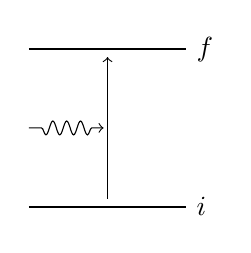
\begin{tikzpicture}%[every node/.style={draw,outer sep=0pt,thick}]

\tikzstyle{spring}=[thick,decorate,decoration={zigzag,pre length=0.3cm,post length=0.3cm,segment length=6}]

\tikzstyle{photon}=[decorate,decoration={snake,pre length=0.15cm,post length=0.15cm,segment length=5}]



\draw [thick] (0,0) -- +(2cm, 0) node [right] {  $\ket{i}$};
\draw [thick] (0,2cm) -- +(2cm, 0) node [right] {  $\ket{f}$};
\draw [->] (1,0.1) -- (1,1.9);

\draw  [<-, photon] (0.95, 1) -- +(-0.95,0);
 
\end{tikzpicture}

